% This file was created by tikzplotlib v0.9.1.
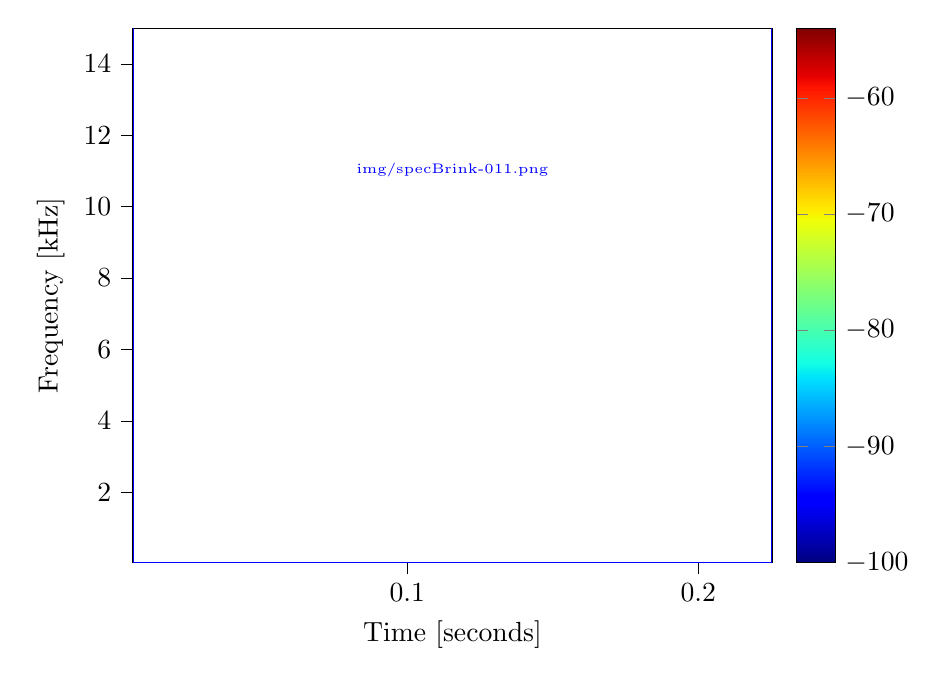
\begin{tikzpicture}

\begin{axis}[
colorbar,
colorbar style={ylabel={}, y label style={yshift=1.5em}},
colormap={mymap}{[1pt]
  rgb(0pt)=(0.0000,0.0000,0.5000);
  rgb(22pt)=(0.0000,0.0000,1.0000);
  rgb(25pt)=(0.0000,0.0000,1.0000);
  rgb(68pt)=(0.0000,0.8600,1.0000);
  rgb(70pt)=(0.0000,0.9000,0.9677);
  rgb(75pt)=(0.0806,1.0000,0.8871);
  rgb(128pt)=(0.9355,1.0000,0.0323);
  rgb(130pt)=(0.9677,0.9630,0.0000);
  rgb(132pt)=(1.0000,0.9259,0.0000);
  rgb(178pt)=(1.0000,0.0741,0.0000);
  rgb(182pt)=(0.9091,0.0000,0.0000);
  rgb(200pt)=(0.5000,0.0000,0.0000)
},
point meta max=-54.0062,
point meta min=-100.0000,
tick align=outside,
tick pos=left,
width=0.8\textwidth,
x grid style={white!69.0196!black},
xlabel={Time [seconds]},
xmin=0.0057, xmax=0.2254,xtick={0.1,0.2},
xtick style={color=black},
y grid style={white!69.0196!black},
ylabel={Frequency [kHz]},
ymin=0.0300000, ymax=15.0000000,
ytick style={color=black}
]
\addplot graphics [includegraphics cmd=\pgfimage,xmin=0.0057, xmax=0.2254, ymin=0.0000, ymax=22.0500000] {img/specBrink-011.png};
\end{axis}

\end{tikzpicture}
